\documentclass[prl,twocolumn,lengthcheck,superscriptaddress]{revtex4-1}

\usepackage{amsmath}
\usepackage{amsthm}
\usepackage{amssymb}
\usepackage{graphicx}
\usepackage{hyperref}
\usepackage{color}
\usepackage{braket}

\newcommand{\tr}{\operatorname{tr}}
\newcommand{\vol}{\operatorname{vol}}
\newcommand{\supp}{\operatorname{supp}}
\newcommand{\dist}{\operatorname{dist}}
\newcommand{\operator}[1]{\ensuremath{\widehat{#1}}}
\newcommand{\ic}{\ensuremath{i}}
\renewcommand{\d}{\ensuremath{d}}
\newcommand{\vx}{\ensuremath{\vec{x}}}
\newcommand{\vk}{\ensuremath{\vec{k}}}

\newtheorem{theorem}{Theorem}
\newtheorem{proposition}{Proposition}
\newtheorem{lemma}{Lemma}
\newtheorem{corollary}{Corollary}

\theoremstyle{definition}
\newtheorem{definition}{Definition}
\newtheorem{example}{Example}

\theoremstyle{remark}
\newtheorem{remark}{Remark}


\begin{document}

\title{Tensor networks and quantum field theory}

\author{Tobias J.\ Osborne}
\affiliation{Institut f\"ur Theoretische Physik, Leibniz Universit\"at Hannover, Appelstr. 2, 30167 Hannover, Germany}

\begin{abstract}
	Here we describe how tensor network states --- a quantum information theory inspired tool originally arising in the study of quantum spin systems --- can be used to understand the physics of quantum fields. In particular, we review the tensor network formalism and outline its application to the study of ground state physics and scattering amplitudes. We describe two approaches, one based on the Lie-Trotter expansion within the hamiltonian formalism, and a second based on the lagrangian formalism which represents the path integral as a tensor network. Our aim in this paper is to present recent developments in condensed matter theory with a quantum field theory audience in mind. 
\end{abstract}

\maketitle

\paragraph{Introduction }\hspace{-1em}.---Quantum field theory is now understood as an effective theory describing the large scale low energy physics \cite{wilson:1975a,wilson:1974a}. By exploiting the correspondence between a statistical physics system at criticality and a quantum field Wilson in one fell swoop resolved all the troubling ``infinities'' plaguing quantum field theory. And so it is that quantum field theory has become a tool par excellence in physics; to understand the large-scale effective physics of any system we need only identify the fixed point --- often uniquely defined by the symmetries of the system --- to which it belongs and, often enough, the resulting QFT describing that situation is amenable to perturbation theory allowed us to deploy the apparatus of Feynman diagrams. 

Tensor network papers: \cite{perez-garcia:2006a}\cite{orus:2013a, evenbly:2011a, evenbly:2009a}\cite{verstraete:2004a}
\cite{vidal:2007a}\cite{levin:2007a}\cite{gu:2009a}


Perturbative QFT is useful and powerful but nonperturbative field theory still contains many mysteries: tantalising hints, via holography, of the power of QFT. Complex network of relationships via holographic duality.

The lattice is a good regulator allowing computers to be brought to bear on deep problems. Amazing insights
\cite{wilson:1974b} from confinement to the hadron spectrum \cite{duerr:2008a}.

The lattice 



The path integral is the way to work with QFT


\cite{horava:2008a}\cite{ardonne:2004a}\cite{horava:2009a}\cite{swingle:2012a}\cite{aharonov:2003a}\cite{rudolph:2002a}\cite{ryu:2006a}\cite{ryu:2006b}\cite{nishioka:2009a}\cite{maldacena:2013a}\cite{hartman:2013a}


Here we must cite Swingle, Vidal, Verstraete, Maldacena, Susskind, Takayanagi etc.....

Important points:
\begin{enumerate}
	\item Path integral formalism to calculate $n$-point functions.
	\item Path integral on the lattice = statistical mechanics.
	\item Method 1: trotter
	\item Method 2: Stat. mech. = lifshitz PEPS.
	\item Scattering amplitudes as $n$-point functions.
	\item Removing the cutoff: 2nd (higher) order phase transition; scaling limit.
	\item Variational calculation of $n$-point functions 
	\item Path integrals+perturbation theory: good for weak coupling bad for strong coupling; TNS good for strong coupling bad for weak.
\end{enumerate}


Since their emergence in 1987 in the condensed matter theory literature there has been an amazing amount of progress in the development of tools, both analytic and numeric, for the study of tensor network states. We cannot do proper justice to the literature here, and we only summarise a couple of the highlights. 

In this paper we argue that tensor network methods are reaching a maturity so that they may be profitably employed as an alternative to the path integral in the study of correlated quantum fields. Here  

In this sense tensor-network methods have become a natural alternative to the path integral appropriate for 

The purpose of this letter is to interpret QFT in the language of tensor networks with a view to formalising possible approaches to studying holographic dualities and the calculation of  To this end we describe two natural approaches to studying the statics and dynamics of QFT via TNS, namely, in the hamiltonian setting familiar to condensed matter theory and a second approach by directly representing the full path integral as a TNS. We then argue how to obtain continuum limits and briefly 

\paragraph{What is a tensor network?}\hspace{-1em}---Tensor networks provide an economic framework to parametrise tensors with many indices. Here we provide a brief overview of the tensor network formalism and sketch some calculational techniques. For some recent reviews of this material see, e.g., \cite{orus:2013a, evenbly:2011a, evenbly:2009a}.

We begin our discussion by considering $n$-index tensors: these are, for us, nothing more than collections $\psi$ of $d_1d_2\cdots d_k$ complex numbers $\psi_{j_1j_2\cdots j_n}$, where $j_k = 1, 2, \ldots, d_k$ and  $d_k$ is the dimension of the index. While we sometimes use the ``upstairs'' and ``downstairs'' notation for indices --- basically in order to unclutter our expressions --- this should not be interpreted as implying that the tensor transforms in any particular way under Lorentz transformations (whose action is not even defined here).

A key device we exploit in the following is to visualise an $n$-index tensor $\psi$ as a vertex (really a circle) with $n$ legs, one for each index $j_k$, $k = 1, 2, \ldots, n$:
\begin{center}
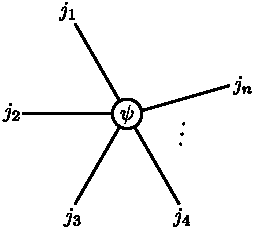
\includegraphics{psitns.pdf}
\end{center}
According to such a visualisation tensors such as vectors are represented as a circle with one leg, matrices as a circle with two legs, and so on:
\begin{center}
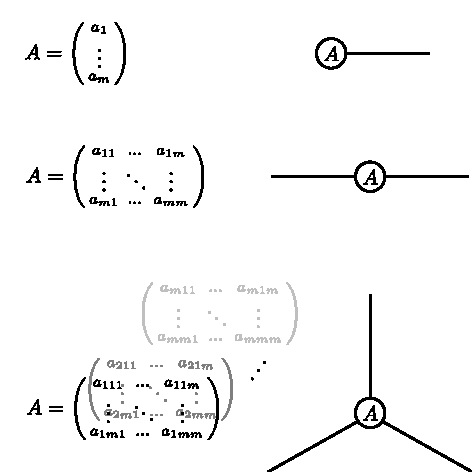
\includegraphics{tns1.pdf}
\end{center}
The contraction of the indices of two tensors is then represented by joining the legs of the corresponding indices. For example:
\begin{center}
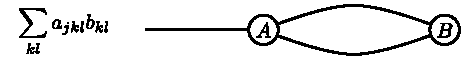
\includegraphics{tns2.pdf}
\end{center}
A \emph{tensor network} is then the tensor $\psi$ associated with a diagram, actually a \emph{graph} $G$, consisting of a collection of tensors, represented as \emph{vertices}, whose indices are contracted according to the \emph{contraction pattern} described by the edges of the graph. The result is a tensor with a number of indices given by the external or ``dangling legs'' of the diagram. 

The canonical example of a tensor network is the \emph{matrix product state} tensor:
\begin{center}
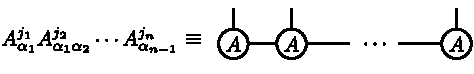
\includegraphics{mps.pdf}
\end{center}

Calculating the value of a tensor network for a given configuration $j_1j_2\cdots j_n$ of the external legs is called \emph{contracting} a tensor network. The problem of contracting, or even approximating the contraction of, an arbitrary tensor network is, in general, \emph{hard}: even \emph{planar} tensor networks can be arbitrarily difficult \cite{schuch:2007a}. Tensor networks are, in general, useful only when they have some additional structure, such as short-ranged correlations (more on this later), topological simplicity, i.e., containing only a few loops, or causal structure, e.g., the tensors are isometries. 


\paragraph{Operations on tensor networks}\hspace{-1em}.---There are a couple of basic operations one can perform on a tensor network to obtain (sometimes simpler) new networks. The first operation is \emph{partial contraction}: here a collection of vertices and their corresponding tensors are identified and the indices corresponding to all the edges connecting these vertices are contracted. The original tensors are then replaced by the resulting amalgamation: 
\begin{center}
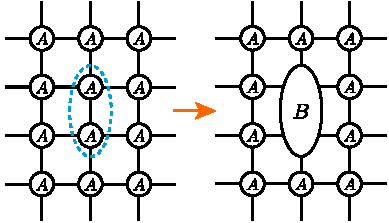
\includegraphics{partialcont.pdf}
\end{center}


The second key primitive is that of \emph{tensor splitting}: here we first collect the external legs of a tensor into two groups which are then regarded as two multi-indices. For example, suppose we have the $n$-index tensor $A$ inside our network: we could collect the first $k$ indices together as the multi index  $\alpha \equiv [j_1j_2 \cdots j_k]$ --- running, say, in lexicographic order through the $d_1d_2\cdots d_k$ assignments of the indices  --- and the remaining indices together as $\beta \equiv [j_{k+1}\cdots j_n]$. This bundling of indices gives us a $2$-index tensor $A_{\alpha\beta}$, where $\alpha$ can be taken to run from $1$ to $d_1\cdots d_k$ and $\beta$ from $1$ to $d_{k+1}\cdots d_n$. We may now regard $A$ as a \emph{matrix}. The tensor splitting operation is then carried out by exploiting the \emph{singular value decomposition} \cite{horn:1990a} to write $A$ as a product of an isometry $U$, a diagonal matrix $d$ with positive entries, and another isometry $V$: 
\begin{equation}\label{eq:svd}
	A = UdV.
\end{equation}
Graphically this is represented as:
\begin{center}
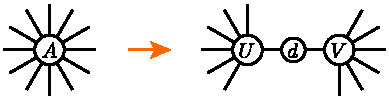
\includegraphics{tensorsplitting.pdf}
\end{center}
Note that the original tensor is replaced with a contraction of three tensors and, in the process, the \emph{degree} of the new vertices in the network is reduced. This procedure may be recursively applied to all the tensors in an arbitrary network to produce a new tensor network with maximal degree bounded above by $3$. (Note: it is impossible, in general, to reduce the degree of all the vertices to $2$ or below via the process.)

The third primitive is \emph{truncation}. Focus on one edge $e$ in a tensor network: this represents a contraction of two specific indices of two tensors. That is, we perform a sum over all the values of the index $\alpha$ indicated by the edge $e$ and shared by the two tensors at the ends of the edge:
\begin{equation}
	\sum_{\alpha = 1}^{d} \cdots A_{\cdots \alpha} B_{\alpha \cdots} \cdots.
\end{equation}
The truncation procedure is an approximation technique where we simply sum over fewer of the possible values of $\alpha$:
\begin{equation}
	\sum_{\alpha = 1}^{d} \cdots A_{\cdots \alpha} B_{\alpha \cdots} \cdots \mapsto \sum_{\alpha = 1}^{d'} \cdots A_{\cdots \alpha} B_{\alpha \cdots} \cdots,
\end{equation}
with $d' < d$. Truncation is particularly effective in combination with tensor splitting: when the diagonal matrix $d$ in Eq.~(\ref{eq:svd}) has many small entries we can simply replace the sum over $\beta$ with a sum over a smaller range, including only the indices corresponding to large entries.

A final approximation operation frequently useful in studying quantum states generated by local dynamics is the \emph{Lie-Trotter} expansion:
\begin{equation}
	e^{A+B} \approx (e^{A/m}e^{B/m})^m,
\end{equation}
where $n$ is a positive integer and $A$ and $B$ are operators on some hilbert space $\mathcal{H}$. This approximation improves as $n$ is increased and becomes an identity in the limit $m\rightarrow \infty$. This result allows us to approximate the propagator $U(t) = e^{-itH}$ --- an $n$-index tensor --- for a quantum spin system with a \emph{local} hamiltonian $H$ by a tensor network involving small-index tensors. To see how this works suppose that $H$ is a hamiltonian for a chain of $n$ quantum spins (similar results hold in higher dimensions):
\begin{equation}
	H = \sum_{j=1}^{n-1} h_j,
\end{equation}
where $h_{j}$ is a local interaction term which acts nontrivially only on spins $j$ and $j+1$. Next collect together the even-numbered (respectively, odd numbered) interactions:
\begin{equation}
	A = \sum_{k=1}^{\lfloor (n-1)/2 \rfloor} h_{2k} \quad \text{and} \quad B = \sum_{k=1}^{\lceil (n-1)/2 \rceil} h_{2k-1}.
\end{equation} 
Now $A$ and $B$ only contain terms which mutually commute with each other, so that $e^{A} = \prod_{k} e^{h_{2k}}$ and $e^{B} = \prod_{k} e^{h_{2k+1}}$. Applying the Lie-Trotter expansion allows us to replace $e^{zH}$ with the product
\begin{equation}
	e^{zH} \approx \left(\prod_{k} e^{\frac{z}{m}h_{2k}}\prod_{k'} e^{\frac{z}{m}h_{2k'}}\right)^m,
\end{equation}
which is a tensor network of $mn$ degree-$4$ tensors. Graphically this is represented by: 
\begin{center}
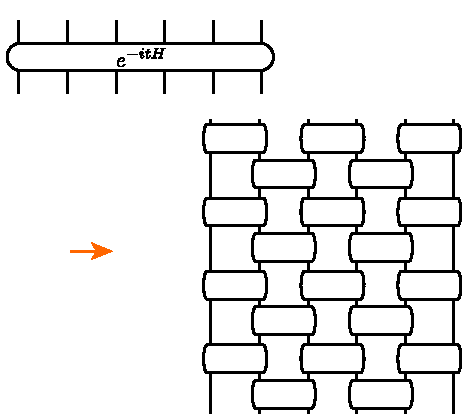
\includegraphics{lietrotter.pdf}
\end{center}
We've thus reduced the contraction of a single degree $2n$ tensor to contracting a network of smaller tensors. In general the difficulty of these two different tasks is roughly equivalent, however, there are cases where the Lie-Trotter network can be exploited to develop useful approximation methods


\paragraph{Tensor network states}\hspace{-1em}.---Tensor network states (TNS) are quantum states of a many body quantum system associated with a tensor network. The systems we typically think about are quantum spin systems comprised of $n$ distinguishable quantum spins with local hilbert spaces $\mathcal{H}_j$, $j = 1, 2, \ldots, n$; the total hilbert space is then $\mathcal{H}\cong \bigotimes_{j=1}^{n} \mathcal{H}_j$. It is common to assume that $\mathcal{H}_j$ is finite dimensional, with dimension $d_j$, although there is no fundamental reason preventing everything from straightforwardly applying to infinite dimensional systems. An arbitrary state $|\psi\rangle$ of $\mathcal{H}$ can be written as
\begin{equation}
	|\psi\rangle = \sum_{j_1 = 1}^{d_1}\cdots \sum_{j_{n} = 1}^{d_{n} } \psi_{j_1j_2 \cdots j_{n}}|j_1\rangle \cdots |j_{n}\rangle,
\end{equation} 
where $|j_k\rangle$ is an arbitrary orthonormal basis for $\mathcal{H}_j$. The state $|\psi\rangle$ is encoded in the $d_1d_2\cdots d_n$ components of the $n$-index tensor $\psi_{j_1j_2 \cdots j_{n}}$.  When the dangling legs of a tensor $\psi$ are associated with an orthonormal basis of a quantum spin system we obtain a \emph{tensor network state}.

\paragraph{Basic properties of tensor network states}\hspace{-1em}.---The tensor network formalism exposes some very powerful structural information about quantum states. 

The first property is that a tensor network state is always manifestly a \emph{state}. This is an extremely useful property not shared by other representations (e.g., a truncated perturbation series around some mixed state does not usually determine a positive state).

The second property is that expectation values of (local) operators may be computed by contracting a related tensor network: let $|\psi\rangle$ be a TNS and $M$ some (local) operator on the $l$th spin. Then the expectation value $\langle M \rangle$ is determined by
\begin{equation}
	 \sum_{j_1 = 1}^{d_1}\cdots\sum_{j_l,k_l = 1}^{d_1} \cdots \sum_{j_{n} = 1}^{d_{n} } \psi^*_{j_1j_2 \cdots j_{n}}\psi_{j_1 \cdots j_{l-1}k_l j_{l+1} \cdots j_{n}} M_{j_lk_l},
\end{equation}
which is the contraction of three tensor networks: one for $\psi^*$, one for $M$, and one for $\psi$.
For example, suppose we have a TNS whose coefficients are determined by the network
\begin{center}
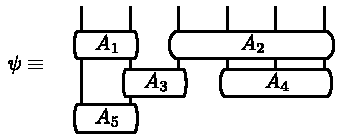
\includegraphics{psinw.pdf}
\end{center}
Then the expectation value of a hermitian operator $M$ on the 3rd spin is given by the contraction
\begin{center}
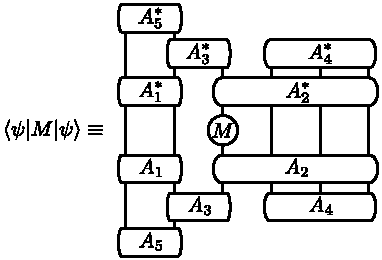
\includegraphics{expvals.pdf}
\end{center}
Closely related to the calculation of expectation values is the construction of the \emph{reduced density operator}. Let $|\psi\rangle$ be a tensor network state. Form the corresponding density operator $\rho \equiv |\psi\rangle\langle \psi|$: this is a tensor network with twice the number of external legs and every tensor doubled. Take the partial trace over all spins outside of region $A$; this operation is found by connecting the indices corresponding to the legs in the complement in $A$ as follows:
\begin{center} 
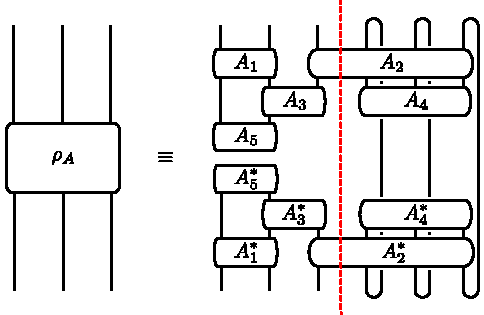
\includegraphics{ptrace.pdf}
\end{center}

The third remarkable property is that we obtain an upper bound on the entropy of entanglement associated a region $\mathcal{R}$ in the network. This result may be argued as follows.  

\paragraph{Tensor networks from hamiltonians}\hspace{-1em}.---


\paragraph{Tensor networks from path integrals}\hspace{-1em}.---

Here we must cite lifschitz theories; ardonne; Horava

The basic input to any calculation in QFT is the lagrangian $\mathcal{L}$. To keep a concrete example in mind think of $\phi^4$ theory in $D+1$ dimensions:
\begin{equation}
	\mathcal{L} = \frac12 (\partial_\mu\phi)^2 - \frac12m^2 \phi^2 -\frac{\lambda}{4!}\phi^4,
\end{equation}
however, everything we discuss here is valid in generality (in particular, everything we say here will apply equally to relativistic and nonrelativistic settings).  Using the lagrangian we can calculate any $n$-point correlation function using the path integral according to the standard formula
\begin{multline}	
	\langle  T[\phi(x_1)\cdots \phi(x_n)] \rangle\equiv\\ \lim_{T\rightarrow \infty(1-i\epsilon)} \frac{\int \mathcal{D}\phi \, \phi(x_1)\cdots \phi(x_n)e^{i\int_{-T}^T d^4x\, \mathcal{L}}}{\int \mathcal{D}\phi\, e^{i\int_{-T}^T d^4x\, \mathcal{L}}}.
\end{multline} 
Before such a path integral can be evaluated --- or even approximated --- it is generally necessary to \emph{regulate} the theory by applying a cutoff $\Lambda$. Now, in the context of tensor networks and quantum information, the most natural regulator is the lattice, with lattice spacing $a = \frac{1}{\Lambda}$, and we don't hesitate to use it throughout. In this way we discretise our continuous field(s) $\phi(x)$ onto the integer lattice $a\mathbb{Z}^{D+1}$; we restrict our coordinates to elements of the form $x_\mu = an_\mu$, $n_\mu \in \mathbb{Z}^{D+1}$. Write the field evaluated at lattice points as $\phi_{n_{\mu}} = \phi(x_\mu)$; thus we discretise derivatives as $\partial_\mu \phi(x_\nu) \mapsto (\phi_{n_\nu + e_{\mu}} - \phi_{n_\nu})/a$,   where $e_\mu$ is the unit lattice vector in the direction $\mu$. Thus our potentially ill-defined path integral becomes the better-behaved iterated integral
\begin{equation}\label{eq:wrcorr}
	\int \mathcal{D}\phi \mapsto \int [d\phi] \equiv \int \left(\prod_{n\in\mathbb{Z}^{D+1}} d\phi_n \right).
\end{equation}
A further important device that we also initially exploit is to make a Wick rotation of time $t\mapsto -i\beta$: this turns our path integral expression for the correlation functions into a statistical mechanical problem:
\begin{equation}	
	\langle  \phi(x_{1}^E)\cdots \phi(x_n^E) \rangle\equiv \frac{1}{\mathcal{Z}}\int [d\phi] \, \phi_{m_1}\cdots \phi_{m_n} e^{-S},
\end{equation} 
where $\mathcal{Z} = \int [d\phi] \, e^{-S}$ and, e.g., $S = a^{D+1}\sum_{\langle m,n\rangle\in \mathbb{Z}^{D+1}} (\phi_m-\phi_n)^2/(2a^2) + \sum_{n} m^2\phi_n^2/2 + \lambda \phi_n^4/4!$.


To practitioners in tensor networks an expression such as Eq.~(\ref{eq:wrcorr}) is strongly suggestive because we can introduce a special pure quantum state $|\Phi\rangle$ which encodes all the information we can extract from a partition function by taking the square root of the probabilities \cite{rudolph:2002a, aharonov:2003a}. The way this works is as follows: if we have a partition function $\mathcal{Z} = \sum_{j=1}^N e^{-E_j}$ for a system with $N$ configurations we introduce the quantum state $|\Phi\rangle \equiv \sum_{j=1}^N e^{-\frac12E_j}|j\rangle/\sqrt{\mathcal{Z}}$, where $|j\rangle$ is an orthonormal basis corresponding to the $N$ possible configurations of the classical system. 

Remarkably, we can also realise $|\Phi\rangle$ as the \emph{ground state} of a natural hamiltonian \cite{ardonne:2004a, verstraete:2006a, perez-garcia:2008a, horava:2008a}. The key to this construction is to introduce a reversible markov chain $M$ which has $p_j \equiv  e^{-E_j}/\mathcal{Z}$ as its stationary distribution \cite{norris:1997a}, i.e., $\sum_{j=1}^N p_jM_{jk} = p_k$, $\forall k$. Reversibility is the condition that $p_j M_{jk} = p_kM_{kj}$, $\forall j,k$. This motivates us to introduce the  matrix with matrix elements:
\begin{equation}
	K_{jk} \equiv \sqrt{p_j} M_{jk} \frac{1}{\sqrt{p_k}}.
\end{equation}
Because of the reversibility condition we find that $K$ is real and symmetric, i.e., hermitian. Further, we have that operator $\widehat{K} \equiv  \sum_{j,k=1}^N K_{jk}|k\rangle \langle j|$ has $|\Phi\rangle$ as an eigenvector corresponding to its largest eigenvalue. We obtain our desired hamiltonian by writing $\widehat{H} \equiv \mathbb{I} - \widehat{K}$, this operator has $|\Phi\rangle$ as a ground state with eigenvalue $0$.

Given a probability distribution of exponential form, i.e., $p_j \equiv  e^{-E_j}/\mathcal{Z}$, there is a special reversible Markov chain having $p_j$ as its stationary distribution, namely, the Metropolis algorithm \cite{metropolis:1953a}. To define this Markov chain we introduce the quantity
\begin{equation}
	c_{jk} \equiv \min\{1, e^{-E_j+E_k}\}.
\end{equation}
Let $F$ be an operator which flips classical configurations, a \emph{flip operator}. In our cases it is convenient to let $F$ be a permutation of $j=1, 2, \ldots, N$. We then use the flip operator to construct
\begin{equation}
	\widehat{M} = \sum_{j\not=k} c_{jk}\langle j|F|k\rangle
\end{equation} 

When we apply the procedure described here to our Wick rotated path integral we obtain the following state of a lattice of a $(D+1)$-dimensional spatial lattice of harmonic oscillators 
\begin{equation}
	|\Phi\rangle \equiv \frac{1}{\mathcal{Z}}\int [d\phi] \,e^{-\frac{S}{2}}  |\boldsymbol{\phi}\rangle,
\end{equation}
where
\begin{equation}
	|\boldsymbol{\phi}\rangle 
\end{equation}

\paragraph{Reflection positivity and analytic continuation}\hspace{-1em}.---

\paragraph{Conclusions}\hspace{-1em}.---The

\bibliography{tnspi}

\end{document}

\widetext
\appendix
\section{$\star$-vector spaces and the Gram-Schmidt procedure}\label{app:ags}
